\subsection{Thread Scheduler}
We describe here an experimence to evaluate the overhead due to thread scheduling.

%\begin{figure*}[h]
%  \centering 
%  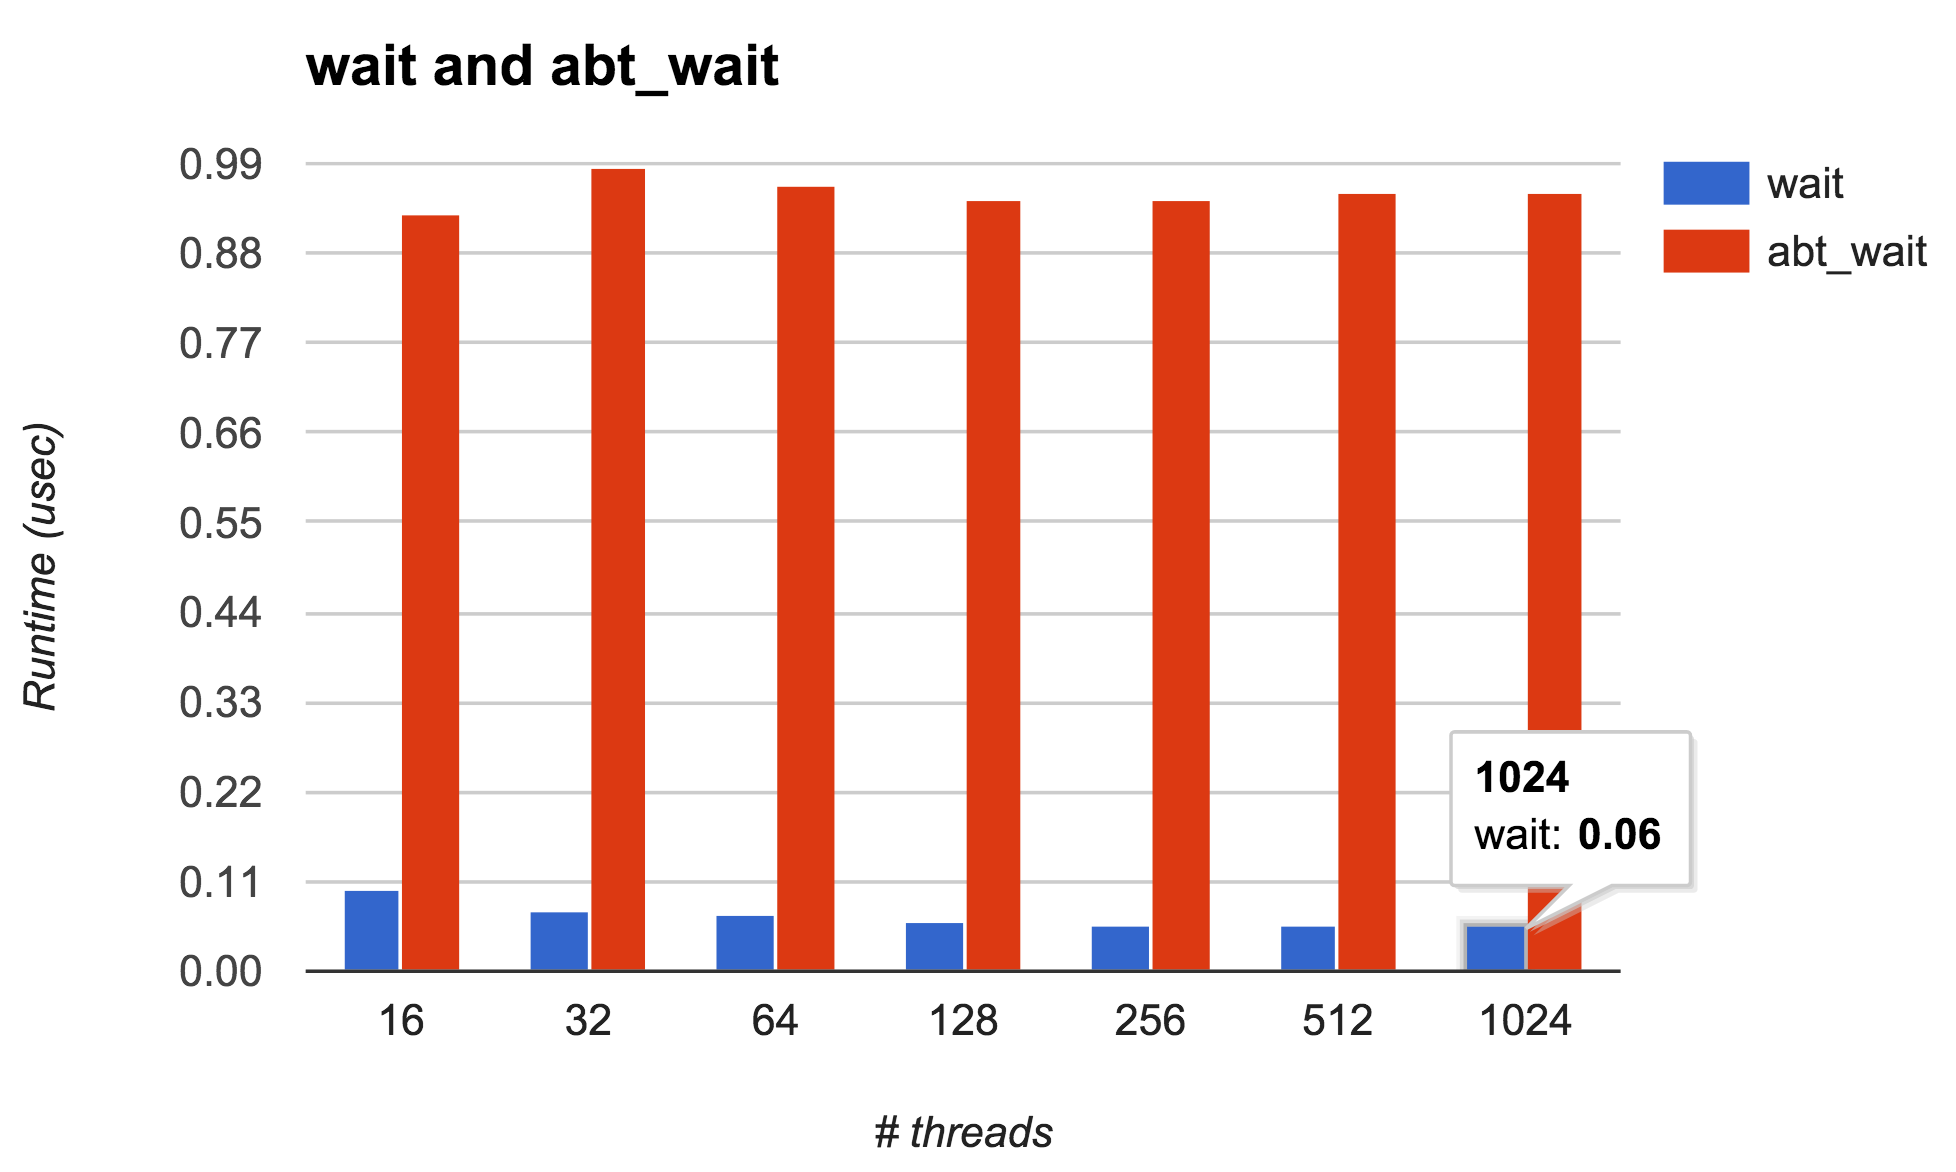
\includegraphics[width=0.6\textwidth]{fig/thread.png}
%  \caption{Comparing Thread wait and signal with Argobots condition variable
%  implementation. Runtime from entering wait until waken up by signal per thread.}
%\end{figure*}

\subsection{Concurrent Hash-Table}
We describe here an experiment to evaluate the overhead due to accessing hash-table.

\subsection{Concurrent Packet Pool}
We describe here an experiment to evaluate the overhead due to packet pool.

%\begin{figure*}[h!]
%  \centering 
%  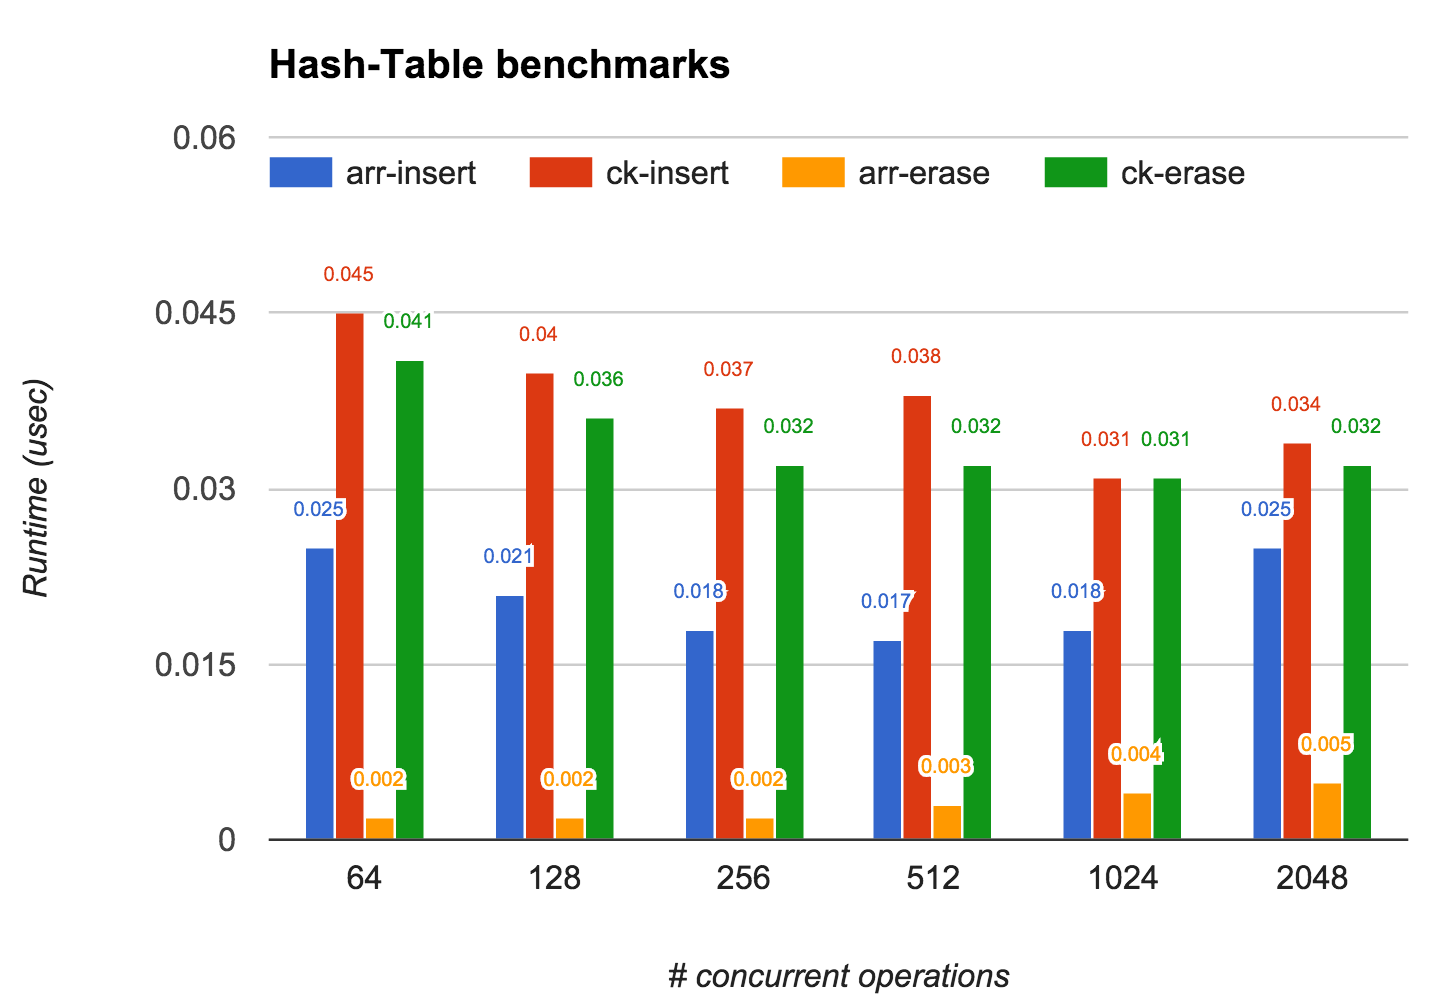
\includegraphics[width=0.6\textwidth]{fig/hashtbl.png}
%  \caption{Comparing hash-table inserting and deletion by concurrent threads
%    with cuckoo-hasing.  Runtime is averaged per operation per thread.
%    \texttt{arr} suffix is our implementation and \texttt{ck} prefix is cuckoo-hasing}.
%\end{figure*}

\subsection{Overall overhead}
Overally this is the overhead.
\begin{figure}[h!]
  \centering 
  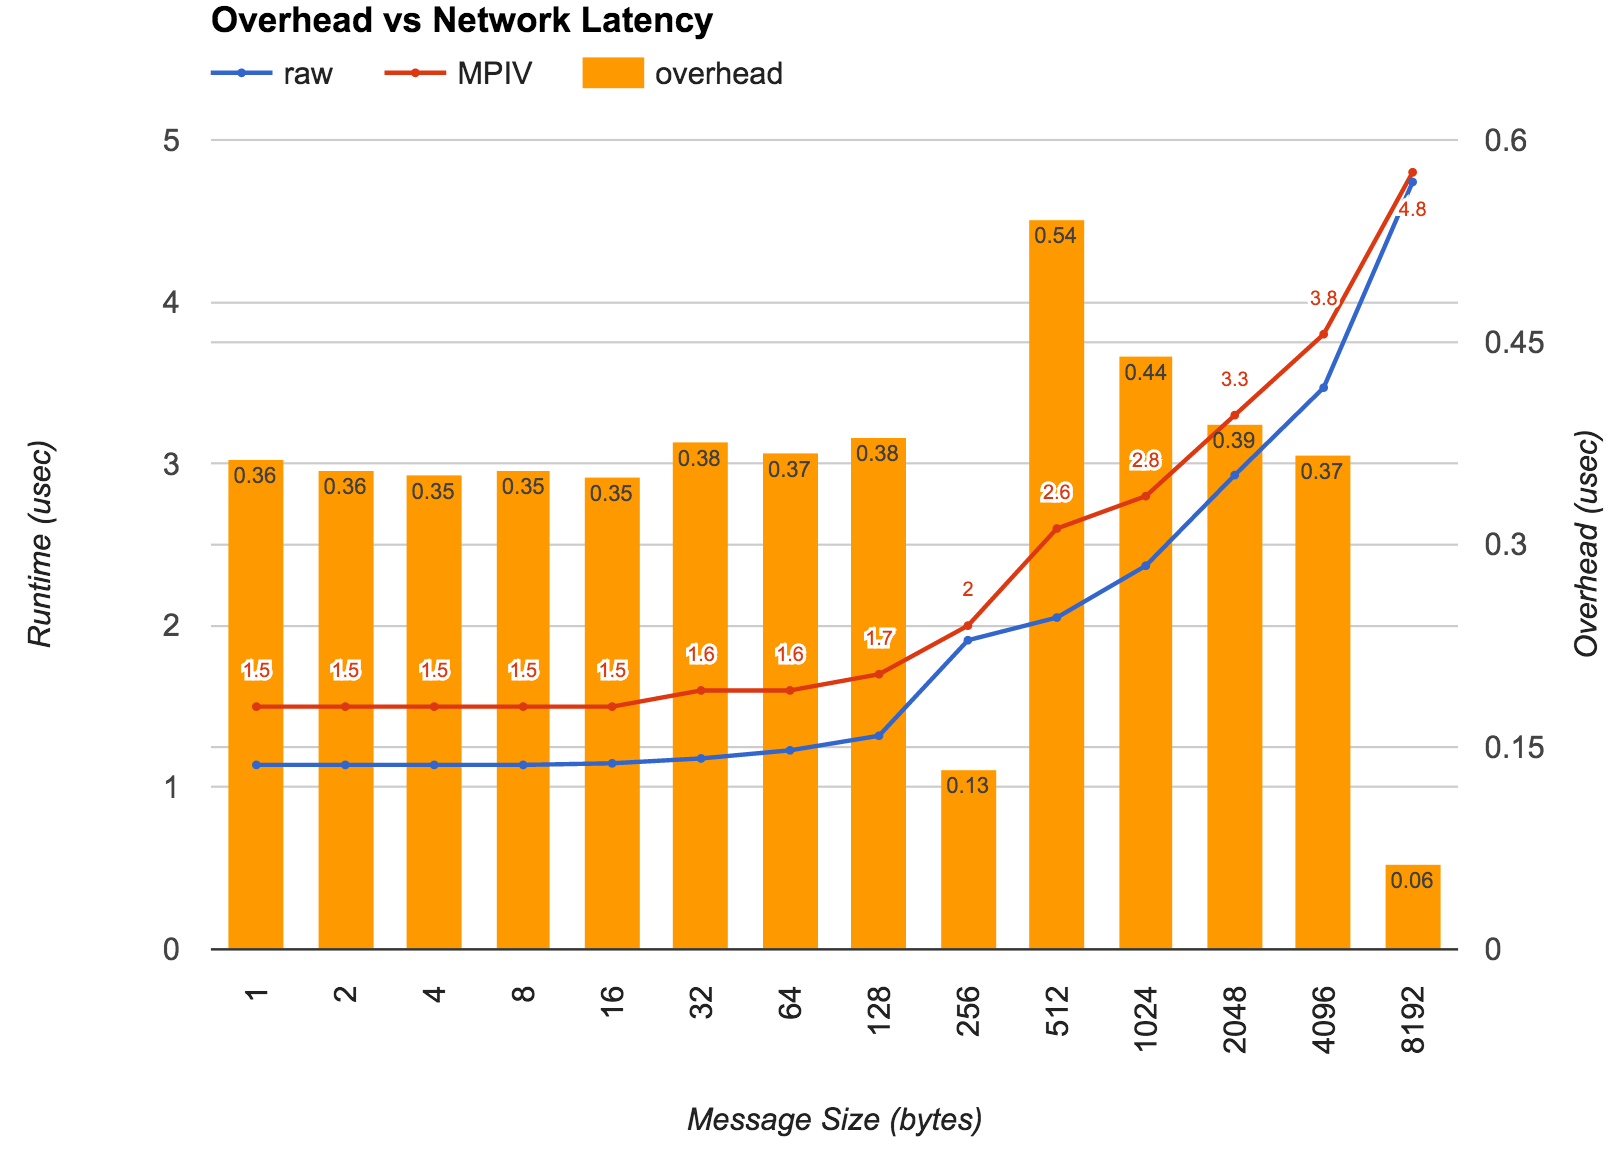
\includegraphics[width=0.2\textwidth]{fig/overhead.png}
  \caption{Total overhead of runtime system, comparing to raw network latency.}
\end{figure}

Overally this is the latency compare to OSU.
\begin{figure}[h!]
  \centering 
  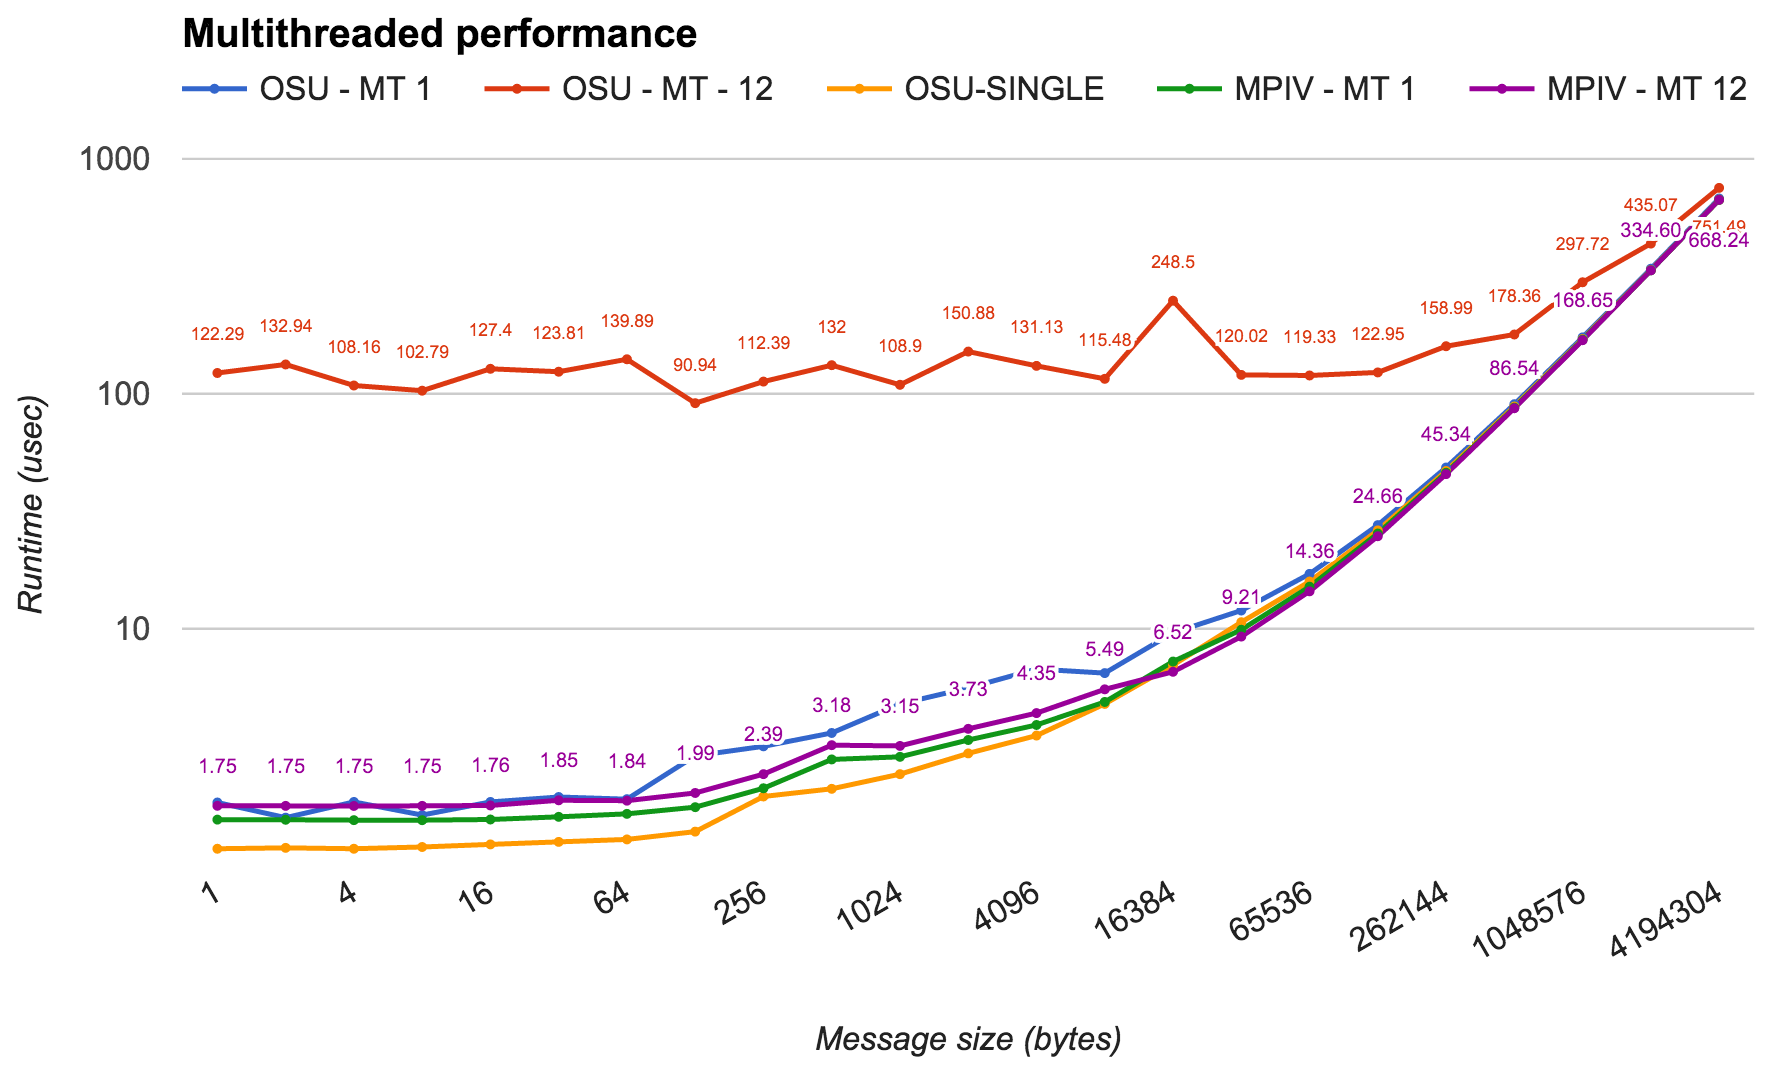
\includegraphics[width=0.2\textwidth]{fig/pingpong.png}
  \caption{Comparing multi-threaded pingpong with OSU benchmarks using 1-thread
  in 1-worker and 12-threads in 12-workers. MPIV is our implementation.}
\end{figure}

Overally this is the message rate compare to OSU.
\begin{figure}[h!]
  \centering 
  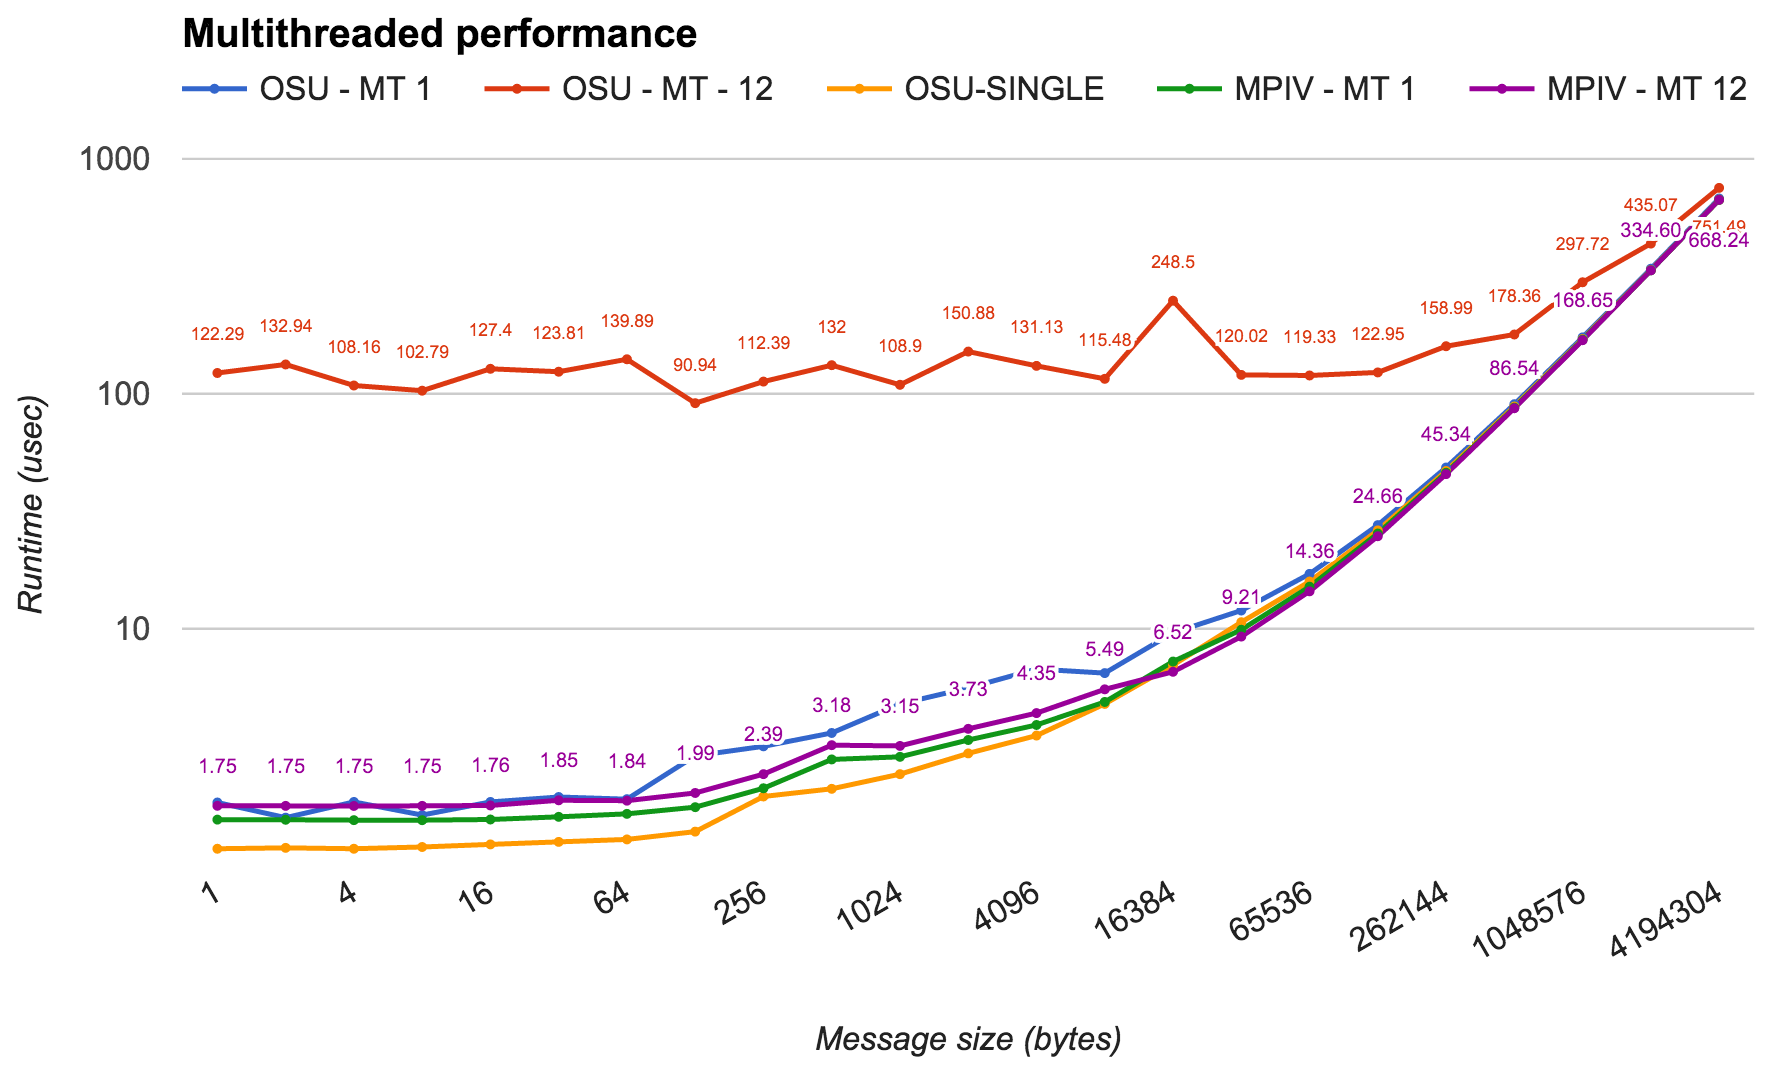
\includegraphics[width=0.2\textwidth]{fig/pingpong.png}
  \caption{Comparing multi-threaded pingpong with OSU benchmarks using 1-thread
  in 1-worker and 12-threads in 12-workers. MPIV is our implementation.}
\end{figure}

\subsection{Applications}
We shows BFS, UTS, Stencil.

